
%
%  $Description: Author guidelines and sample document in LaTeX 2.09$ 
%
%  $Author: ienne $
%  $Date: 1995/09/15 15:20:59 $
%  $Revision: 1.4 $
%

\documentclass[times, 10pt,twocolumn]{article} 
\usepackage{latex8}
\usepackage{times}
\usepackage{graphicx}
\usepackage{epstopdf}

%\documentstyle[times,art10,twocolumn,latex8]{article}

%------------------------------------------------------------------------- 
% take the % away on next line to produce the final camera-ready version 
\pagestyle{empty}

%------------------------------------------------------------------------- 
\begin{document}

\title{Distributed Software Transactional Memory}

\maketitle
\thispagestyle{empty}

\begin{abstract}


   The present paper describes the details of a distributed software
   transactional memory implementation.
   There are 2 scenarios presented for a Master/Server architecture: \\
   a) perfect links and processes (Master and Servers) \\
   b) perfect links and Master, but recoverable Servers \\

   Transaction management, concurrency control, failure detector and 
   replication mechanisms are described for both perfect and fault-tolerant
   architectures.
   
\end{abstract}



%------------------------------------------------------------------------- 
\Section{Introduction}
In the following sections the implementation of a distributed software 
transactional memory library is presented for two scenarios:\\
a) perfect Master, Servers and links\\
b) perfect Master, links and recoverable, sequentially consistent Servers\\

Section \ref{sec:arch} introduces an overview of each scenario. Section 
\ref{sec:algor} discusses the algorithms used for concurrency control, 
transaction management and Client-Server communication


%------------------------------------------------------------------------- 
\Section{Architecture}
\label{sec:arch}

%TODO: Include diagram for both scenarios in different subsections.

%------------------------------------------------------------------------- 
\SubSection{Perfect links and processes}
\label{subsec:perf}
As illustrated in Figure \ref{fig:perf}, the architecture consists of the 
following perfect entities: 
\begin{itemize}
\item {\bf M} - Master server 
\item {\bf S} - Object server
\item {\bf C} - Client      
\end{itemize}

\begin{figure}
\centering
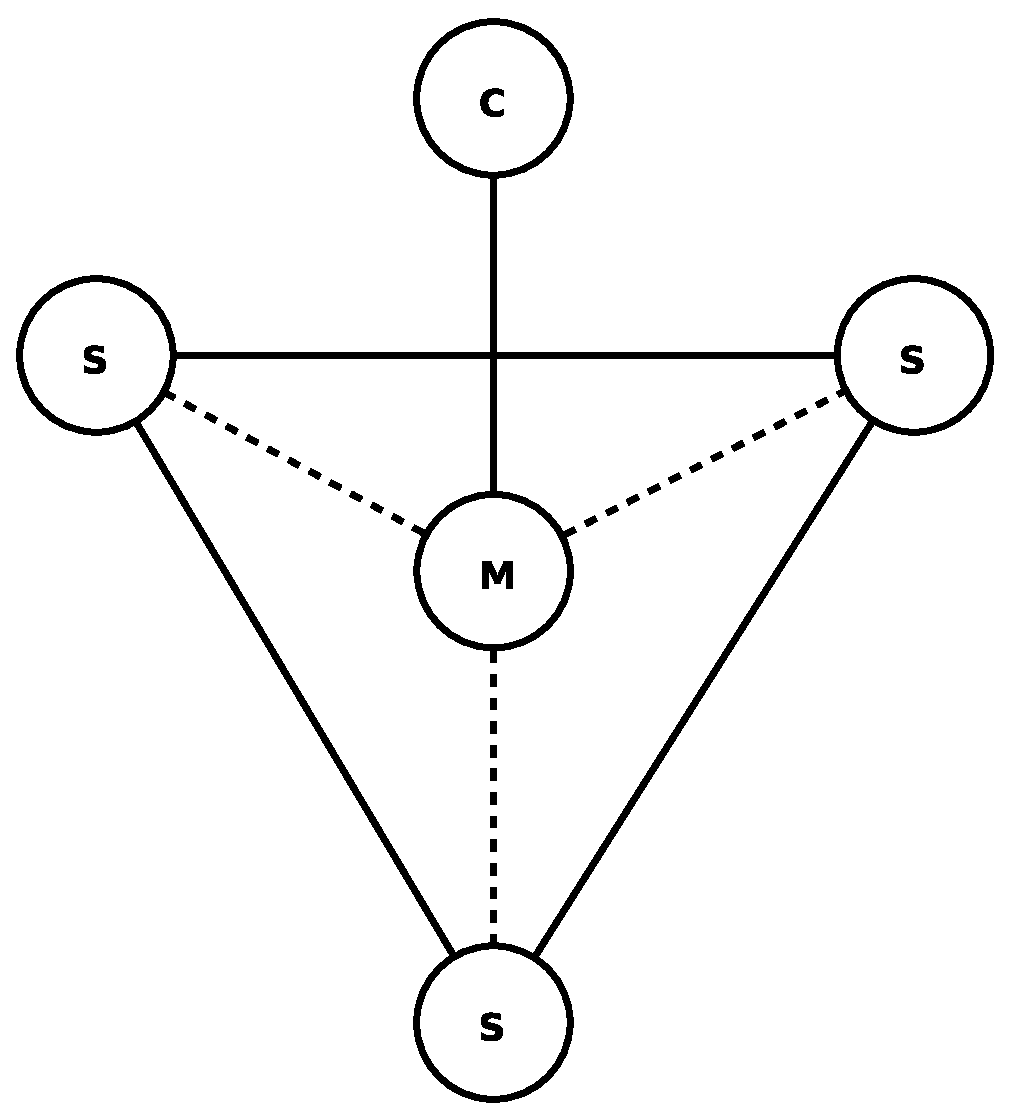
\includegraphics[scale=0.3]{perfect.eps}
\caption{Perfect nodes and links for Master/Server entities}
\label{fig:perf}
\end{figure}
Note that the number of object servers can be varied.
%------------------------------------------------------------------------- 
\SubSection{Recoverable, replicated Servers with perfect Master}
\label{subsec:recov}

%------------------------------------------------------------------------- 
\Section{Algorithms}
\label{sec:algor}

%------------------------------------------------------------------------ 
\SubSection{Communication}
The following communication occurs {\bf before} the client attempts connection 
to the Master node.
\begin{enumerate}
\item Master starts first followed by the Object Servers bootstrap
\item During Object Servers bootstrap:
\begin{enumerate}
\item Master identifies the Object Servers trying to connect
\item Master assigns a unique name to the Object Servers for later use as a reference
\end{enumerate}
\item Object Servers's heartbeat messages periodically sent to Master. This is useful for replica management i.e. If one of the replicas fail then the objects can be replicated in another replica to always maintain a certain level of availability in the system.
\end{enumerate}

Upon {\bf attempting a transaction} (object storage) the following communication exists between the Client, the Master and Object Servers:

\begin{enumerate}
\item Client connects to the Master and requests a transaction identifier 
\item Master maintains a global transaction sequence and returns a unique transaction identifier (TID) to the Client. Furthermore, a list of healthy Object Servers is also returned to the Client to cache for future reference.
\item Client generates a unique ID (integer) when generating the object and client apply the modulo function for the unique id and decide the server, where the object needs to be saved.
\item Client uses the modulo result to connect to the Object Server and store the object representing the tentative versions of the transaction.
\end{enumerate}

When the Client attempts to {\bf manipulate an existing object} in the {\it perfect} Object Servers, the following communication takes place:
\begin{enumerate}
\item Client requests and retrieves TID from Master
\item Client retrieves object's previously generated unique ID
\item Client applies modulo on the retrieved ID to locate the relevant Object Server to request for reference
\item With the retrieved object reference, client can manipulate the object value
\end{enumerate}

%------------------------------------------------------------------------- 
\SubSection{Transaction Management and Concurrency Control}
\label{subsec:transmgt}
The {\it Flat Transaction} model allows for a client to manipulate objects on multiple servers in a single transaction. With regards to concurrency control {\it Timestamp Ordering} is being chosen.

The advantages of choosing {\it Timestamp Ordering} over {\it Two-Phase Locking} or {\it Optimistic Concurrency} options are the following: 
\begin{itemize}
\item Deadlock prevention - common with the use of locks
\item Better performance for transactions with predominantly {\it read} operations \cite{bernstein1987concurrency}
\item Faster conflict resolution when compared to locking - transactions are aborted immediately.
\end{itemize}

The following steps are made when performing a transaction: 
\begin{enumerate}
\item Client acquires transaction ID from the Master
\item Client passes TID to the Object Server
\item Object Server calls the Coordinator's(Master's) {\it join()} method along with TID as parameter
\item Client manipulates objects directly on the Object Server
\item Upon transaction end, Client asks the Coordinator to either {\it Abort} or {\it Commit} 
\item Coordinator will request each participant server in the transaction to indicate whether it can commit a transaction or not.
\item If all participants answer {\it yes}, Coordinator issues {\bf doCommit(TID)} command such that each parcipant commits its part of the transaction
\item Once completed, all servers acknowledge the commit and Coordinator notifies the Client that it's successful.
\item Should any of the participant servers be unable or disagree to commit and aborts, the Coordinator will request all the remaining participants to abort. Client will then be notified.
\end{enumerate}

%-------------------------------------------------------------------------
\SubSection{Timestamp Ordering and Deadlock Detection}
\label{subsec:dldetect}
Since timestamp ordering will be used for concurrency control the chances of deadlock appearing are eliminated.
Each transaction is assigned a unique timestamp value when it starts. Each operation in a transaction is validated when it is carried out.
If a transaction fails the validation, it is aborted immediately and can then be started by the client. The client is issued with a globally unique transaction timestamp by the first coordinator accessed
by a transaction. The servers are jointly responsible for ensuring serial equivalence i.e. if server S1 access an object before server S2, then server S1 is before S2 at all objects. The coordinators
must agree on timestamp ordering so as to achieve the same ordering at all the servers. The timestamp will consist of a {\it <local timestamp, server-id> } pair. Timestamps can be kept roughly synchronized
by the use of synchronized local physical clocks coordinated by the master.

Conflict resolution will be performed at each operation.
The basic timestamp ordering rule is based on operation conflicts and is very simple:
{\it A transaction’s request to write an object is valid only if that object was last read and written by earlier transactions. A transaction’s request to read an object is valid only if that object was
last written by an earlier transaction.} [Reference: Distributed Systems].
If the resolution is to abort the transaction then the coordinator will be informed and it will abort the transaction at all the participants.

%--------------------------------------------------------------------------
\SubSection{Fault Tolerance}
\label{subsec:faultol}
In this phase we design to provide fault tolerance for single object server failure. This is an extension for the previous design. The idea is to keep an exact copy of the objects in adjacent server.
For instance the object stored in Object server S1, should keep the exact copy in the S2 server as a replica. The master server is responsible for keeping track of the replica servers.

When the object server {\bf fails},
\begin{enumerate}
\item Master detects the server failure from the absence of the heartbeat message from the object server.
\item Master server issues a {\it “failure warning notification”} for the servers, so that the current transactions related to the absent server will be aborted.
Others will continue but new transactions will not be proceeded. (Master block providing TIDs)
\item Master server coordinates object replication so that the currently available servers share the objects held by the absent server.
\item Once the master notifies all the servers about the stabilized status, transactions can be continued again.
\end{enumerate}

When the failed server {\bf recovers},
\begin{enumerate}
\item Master detects the arrival of a new server.
\item Master server issues a {\it “New server notification”} for the servers. Once the current pending transactions are completed, stabilizing the servers occur.
\item Master server coordinates object replication so that the currently available servers share the objects held by the absent server.
\item Once the master notifies all the servers the stabilized status, transactions can be continued again.
\end{enumerate}

%------------------------------------------------------------------------- 
\Section{Footnotes}

Please use footnotes sparingly%
\footnote
   {%
     Or, better still, try to avoid footnotes altogether.  To help your 
     readers, avoid using footnotes altogether and include necessary 
     peripheral observations in the text (within parentheses, if you 
     prefer, as in this sentence).
   }
and place them at the bottom of the column on the page on which they are 
referenced. Use Times 8-point type, single-spaced.


%------------------------------------------------------------------------- 
\SubSection{References}

%------------------------------------------------------------------------- 
\SubSection{Conclusions}

%------------------------------------------------------------------------- 
\bibliographystyle{latex8}
\bibliography{latex8}

\end{document}

